\documentclass[tikz,border=7pt]{standalone}
\usepackage{amsmath,amssymb}
\usetikzlibrary{arrows.meta,positioning}
\tikzset{vertex/.style={circle,draw,fill=cyan!12,minimum size=7mm,inner sep=1pt},box/.style={draw,rounded corners,fill=cyan!8,align=center,minimum height=12mm,minimum width=27mm}}
\begin{document}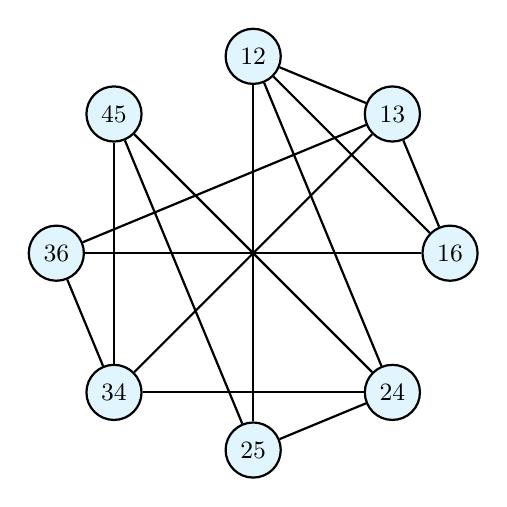
\begin{tikzpicture}[line width=0.8pt,font=\small]
\node[vertex] (v1) at (0.0,2.5) {$12$};
\node[vertex] (v2) at (1.7678,1.7678) {$13$};
\node[vertex] (v3) at (2.5,0.0) {$16$};
\node[vertex] (v4) at (1.7678,-1.7678) {$24$};
\node[vertex] (v5) at (0.0,-2.5) {$25$};
\node[vertex] (v6) at (-1.7678,-1.7678) {$34$};
\node[vertex] (v7) at (-2.5,-0.0) {$36$};
\node[vertex] (v8) at (-1.7678,1.7678) {$45$};
\draw (v1) -- (v2);
\draw (v1) -- (v3);
\draw (v1) -- (v4);
\draw (v1) -- (v5);
\draw (v2) -- (v3);
\draw (v2) -- (v6);
\draw (v2) -- (v7);
\draw (v3) -- (v7);
\draw (v4) -- (v5);
\draw (v4) -- (v6);
\draw (v4) -- (v8);
\draw (v5) -- (v8);
\draw (v6) -- (v7);
\draw (v6) -- (v8);
\end{tikzpicture}\end{document}
